\documentclass[10pt,aspectratio=169]{beamer}

% ---------- Theme ----------
\usetheme[numbering=fraction,progressbar=frametitle]{metropolis}
\usepackage[T1]{fontenc}
\usepackage[utf8]{inputenc}
\usepackage{sourcesanspro}
\usepackage{sourcecodepro}
\usefonttheme{professionalfonts}
\usepackage{amsmath,amssymb,mathtools}
\usepackage{booktabs}
\usepackage{array}
\usepackage{multirow}
\usepackage{ragged2e}
\usepackage{tikz}
\usetikzlibrary{arrows.meta,positioning,calc,fit,backgrounds,matrix,shapes.geometric,decorations.pathreplacing}
\usepackage{xcolor}
\usepackage{listings}
\usepackage{pgfpages}
\usepackage{appendixnumberbeamer}
\usepackage{hyperref}

% ---------- Colors ----------
\definecolor{DeepNavy}{HTML}{183247}
\definecolor{Steel}{HTML}{466A80}
\definecolor{Teal}{HTML}{148A96}
\definecolor{Orange}{HTML}{D97732}
\definecolor{SoftRed}{HTML}{B64B4B}
\definecolor{Ink}{HTML}{1D252C}
\definecolor{Mist}{HTML}{EEF3F5}
\definecolor{MidGray}{HTML}{6B747B}
\definecolor{LightGray}{HTML}{D7DEE2}
\definecolor{Success}{HTML}{2E7D5B}

\setbeamercolor{normal text}{fg=Ink,bg=white}
\setbeamercolor{frametitle}{fg=DeepNavy,bg=white}
\setbeamercolor{progress bar}{fg=Teal,bg=LightGray}
\setbeamercolor{progress bar in head/foot}{fg=Teal,bg=LightGray}
\setbeamercolor{title separator}{fg=Teal}
\setbeamercolor{alerted text}{fg=Orange}
\setbeamercolor{block title}{fg=white,bg=DeepNavy}
\setbeamercolor{block body}{fg=Ink,bg=Mist}
\setbeamercolor{example text}{fg=Teal}
\setbeamercolor{footline}{fg=MidGray,bg=white}

\setbeamerfont{title}{size=\Large,series=\bfseries}
\setbeamerfont{subtitle}{size=\large}
\setbeamerfont{frametitle}{size=\Large,series=\bfseries}
\setbeamerfont{footnote}{size=\tiny}
\setbeamersize{text margin left=0.65cm,text margin right=0.65cm}

% ---------- Listings ----------
\lstset{
  basicstyle=\ttfamily\small,
  keywordstyle=\bfseries\color{DeepNavy},
  commentstyle=\color{MidGray},
  frame=single,
  rulecolor=\color{LightGray},
  backgroundcolor=\color{Mist!55},
  framerule=0.4pt,
  xleftmargin=0.4em,
  xrightmargin=0.4em,
  aboveskip=0.4em,
  belowskip=0.4em,
  showstringspaces=false,
  columns=fullflexible
}

% ---------- Reusable helpers ----------
\newcommand{\emphbox}[1]{%
  \begin{beamercolorbox}[wd=\linewidth,sep=0.55em,rounded=true]{block body}%
  \centering\bfseries\color{DeepNavy}#1
  \end{beamercolorbox}}

\newcommand{\takeaway}[1]{%
  \par\vspace{0.20em}
  \begin{beamercolorbox}[wd=\linewidth,sep=0.34em,rounded=true]{block body}%
  \centering\normalsize\bfseries\color{DeepNavy}#1
  \end{beamercolorbox}}

\newcommand{\smallsource}[1]{\par\vspace{0.3em}{\scriptsize\color{MidGray}#1}}
\newcommand{\yes}{\textcolor{Success}{\bfseries +}}
\newcommand{\no}{\textcolor{SoftRed}{\bfseries -}}

% Notes are embedded in the .tex but hidden in the normal PDF.
\ifdefined\seminarnotes
  \setbeameroption{show notes on second screen=right}
\else
  \setbeameroption{hide notes}
\fi

% ---------- Metadata ----------
\title{Finding Regularity: High-Performance Computing for Graph Algorithms}
\subtitle{High-performance computing and parallel algorithms}
\author{Gökhan Göktürk}
\institute{Computer Science}
\date{}



\begin{document}

% MAIN 01 | 20 seconds | cumulative 0:20
\begin{frame}[plain]{}
\relax
{\Large\bfseries\color{DeepNavy}Finding Regularity:\par
High-Performance Computing for Graph Algorithms\par}
\par\vspace{0.7cm}
{\large Gökhan Göktürk\par}
\par\vspace{0.2cm}
High-performance computing and parallel algorithms\par
\par\vspace{0.6cm}
{\color{Teal}\rule{\linewidth}{0.8pt}}\par
Computer Science Seminar
\end{frame}

\note{\small\textbf{Slide 1: 20 seconds; finish at 0:20.} Open with the research question; graphs are the concrete domain. Introduce execution order, representation, and hardware mapping without reading the title.}

% MAIN 02 | 30 seconds | cumulative 0:50
\begin{frame}{Research background}
\relax
\textbf{Sabancı University}\par
BSc · MSc · PhD · PostDoc
\par\vspace{0.5cm}
\begin{columns}[T,onlytextwidth]
\column{0.48\textwidth}
\textbf{Research}
\begin{itemize}
  \item High-performance computing
  \item Parallel and distributed algorithms
  \item GPU and multi-GPU computing
  \item Graph and probabilistic algorithms
  \item Performance engineering
\end{itemize}
\column{0.47\textwidth}
\textbf{Technical consulting}
\begin{itemize}
  \item Şişecam
  \item Akbank
  \item Sigorta Bilgi Merkezi
  \item Aksigorta
\end{itemize}
\end{columns}
\end{frame}

\note{\small\textbf{Slide 2: 30 seconds; finish at 0:50.} Summarize the academic path and research scope. Mention consulting collectively; do not read every organization aloud.}

% MAIN 03 | 50 seconds | cumulative 1:40
\begin{frame}{High-Performance Computing (HPC)}
\relax
Designing \textbf{algorithms and systems} to solve
demanding computational problems efficiently.
\par\vspace{0.3cm}
\begin{itemize}
  \item \textbf{Reducing work:} exploiting mathematical structure, avoiding redundant computation, reusing intermediate results.
  \item \textbf{Changing representation:} sparse formats, compressed data, compact sketches.
  \item \textbf{Reformulating computation:} batching, fusion, blocking, and different execution orders.
  \item \textbf{Managing accuracy--cost tradeoffs:} approximation, sampling, or reduced precision when the application permits them.
\end{itemize}
\par\vspace{0.25cm}
\textbf{Hardware:} multicore CPUs and vector units · GPUs and other accelerators · clusters
\par\vspace{0.25cm}
\takeaway{The goal: solve larger problems in less time with the available resources.}
\end{frame}

\note{\small\textbf{Slide 3: 50 seconds; finish at 1:40.} Explain the four algorithmic choices without reading every example. Connect them to CPUs, vector units, GPUs, and clusters. End with the trade of extra arithmetic for less data movement.}

% MAIN 04 | 90 seconds | cumulative 3:10
\begin{frame}{Why parallelism is not automatically performance}
\relax
A \textbf{lane} is one position in a group performing an operation in parallel.
\par\vspace{0.25cm}
\begin{columns}[T,onlytextwidth]
\column{0.48\textwidth}
\centering\textbf{Regular array update: $y[i]=2x[i]$}\par\vspace{0.15cm}
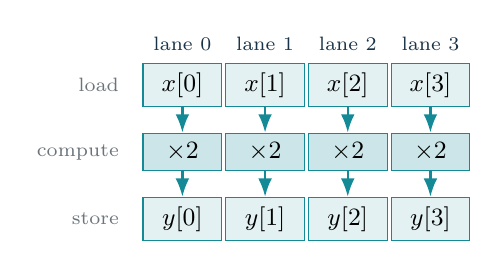
\begin{tikzpicture}[x=1.05cm,y=0.85cm,>=Latex,every node/.style={font=\small}]
  \node[anchor=east,font=\scriptsize,text=MidGray] at (-0.65,2) {load};
  \node[anchor=east,font=\scriptsize,text=MidGray] at (-0.65,1) {compute};
  \node[anchor=east,font=\scriptsize,text=MidGray] at (-0.65,0) {store};
  \foreach \i in {0,...,3}{
    \node[font=\scriptsize,text=DeepNavy] at (\i,2.62) {lane \i};
    \node[draw=Teal,fill=Teal!12,minimum width=1.0cm,minimum height=0.48cm] (x\i) at (\i,2) {$x[\i]$};
    \node[draw=Teal,fill=Teal!22,minimum width=1.0cm,minimum height=0.48cm] (op\i) at (\i,1) {$\times 2$};
    \node[draw=Teal,fill=Teal!12,minimum width=1.0cm,minimum height=0.48cm] (y\i) at (\i,0) {$y[\i]$};
    \draw[->,thick,Teal] (x\i)--(op\i);
    \draw[->,thick,Teal] (op\i)--(y\i);
  }
\end{tikzpicture}
\par\vspace{0.15cm}
\textcolor{Teal}{\textbf{Predictable, direct access}\\Adjacent array elements; equal work per lane.}
\column{0.48\textwidth}
\centering\textbf{Graph traversal: data-dependent addresses}\par\vspace{0.15cm}
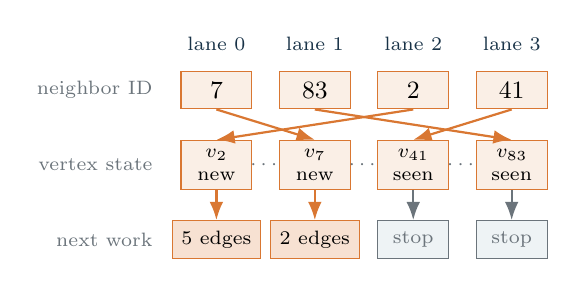
\begin{tikzpicture}[x=1.25cm,y=0.95cm,>=Latex,every node/.style={font=\small,align=center}]
  \node[anchor=east,font=\scriptsize,text=MidGray] at (-0.55,2) {neighbor ID};
  \node[anchor=east,font=\scriptsize,text=MidGray] at (-0.55,1) {vertex state};
  \node[anchor=east,font=\scriptsize,text=MidGray] at (-0.55,0) {next work};
  \foreach \i/\v in {0/7,1/83,2/2,3/41}{
    \node[font=\scriptsize,text=DeepNavy] at (\i,2.62) {lane \i};
    \node[draw=Orange,fill=Orange!12,minimum width=0.9cm,minimum height=0.48cm] (id\i) at (\i,2) {$\v$};
  }
  \foreach \i/\v/\status in {0/2/new,1/7/new,2/41/seen,3/83/seen}{
    \node[draw=Orange,fill=Orange!12,minimum width=0.9cm,minimum height=0.57cm,font=\scriptsize] (st\i) at (\i,1) {$v_{\v}$\\\status};
  }
  \foreach \x in {0.5,1.5,2.5}{\node[font=\scriptsize,text=MidGray] at (\x,1) {$\cdots$};}
  \draw[->,thick,Orange] (id0.south)--(st1.north);
  \draw[->,thick,Orange] (id1.south)--(st3.north);
  \draw[->,thick,Orange] (id2.south)--(st0.north);
  \draw[->,thick,Orange] (id3.south)--(st2.north);
  \foreach \i/\work in {0/5 edges,1/2 edges}{
    \node[draw=Orange,fill=Orange!22,minimum width=0.9cm,minimum height=0.48cm,font=\scriptsize] (work\i) at (\i,0) {\work};
    \draw[->,thick,Orange] (st\i)--(work\i);
  }
  \foreach \i in {2,3}{
    \node[draw=MidGray,fill=Mist,minimum width=0.9cm,minimum height=0.48cm,font=\scriptsize,text=MidGray] (work\i) at (\i,0) {stop};
    \draw[->,thick,MidGray] (st\i)--(work\i);
  }
\end{tikzpicture}
\par\vspace{0.15cm}
\textcolor{Orange}{\textbf{Unpredictable, indirect access}\\Scattered vertex state; unequal work per lane.}
\end{columns}
\par\vspace{0.2cm}
\takeaway{More lanes help when data access and work distribution keep them productive.}
\end{frame}

\note{\small\textbf{Slide 4: 90 seconds; finish at 3:10.} Define a lane. Explain the array example briefly. Trace only lane 0 to vertex 7 (two edges) and lane 1 to vertex 83 (already seen, stop). Mention that another lane has five edges. Pause for the audience to follow the arrows. Conclude with memory stalls and idle lanes.}

% MAIN 05 | 35 seconds | cumulative 3:45
\begin{frame}{The research question}
\relax
{\Large\bfseries\color{DeepNavy}
How can we reorganize irregular computation so that modern parallel hardware can execute it efficiently?\par}
\par\vspace{0.3cm}
\textbf{Regularity:} predictable memory access and similar work across parallel lanes.
\par\vspace{0.3cm}
\renewcommand{\arraystretch}{1.3}
\begin{tabular}{@{}>{\raggedright\arraybackslash}p{4.0cm}>{\raggedright\arraybackslash}p{9.1cm}@{}}
\textbf{What can I change?} & \textbf{What can it improve?}\\
\midrule
Which work runs together & Reuse data; bring memory accesses closer together.\\
What state is stored & Reduce the memory footprint; make updates uniform.\\
Where work executes & Match work to CPU, GPU, and device-local memory.
\end{tabular}\par
\par\vspace{0.3cm}
\textbf{Each change must preserve} the required result, sampling distribution, or accuracy target.
\end{frame}

\note{\small\textbf{Slide 5: 35 seconds; finish at 3:45.} Define regularity as predictable memory access and similar work across parallel lanes. Useful structure may be partial or temporary. Explain the three choices and the result, sampling, or accuracy requirement.}

% MAIN 06 | 80 seconds | cumulative 5:05
\begin{frame}{Running example: influence maximization}
\relax
\begin{columns}[T,onlytextwidth]
\column{0.48\textwidth}
{\small\textbf{Which $k$ seeds maximize their combined influence?}\par
Spread is stochastic; influence overlaps.\par}
\vspace{0.15cm}
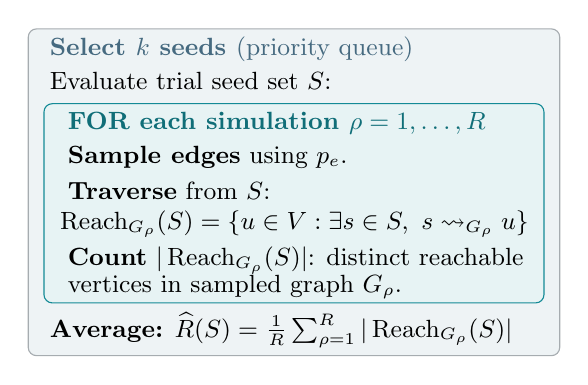
\begin{tikzpicture}[x=1cm,y=1cm,>=Latex,every node/.style={font=\small,anchor=west}]
  \draw[MidGray!60,fill=Mist,rounded corners=3pt] (0,0) rectangle (6.75,-4.15);
  \node[text=Steel,font=\small\bfseries] at (0.15,-0.26) {Select $k$ seeds \textnormal{(priority queue)}};
  \node at (0.15,-0.66) {Evaluate trial seed set $S$:};
  \draw[Teal,fill=Teal!10,rounded corners=3pt] (0.2,-0.95) rectangle (6.55,-3.48);
  \node[text=Teal!80!black,font=\small\bfseries] at (0.38,-1.2) {FOR each simulation $\rho=1,\ldots,R$};
  \node at (0.38,-1.63) {\textbf{Sample edges} using $p_e$.};
  \node at (0.38,-2.06) {\textbf{Traverse} from $S$:};
  \node[anchor=center] at (3.38,-2.48)
    {$\operatorname{Reach}_{G_\rho}(S)=\{u\in V:\exists s\in S,\ s\leadsto_{G_\rho}u\}$};
  \node at (0.38,-2.94) {\textbf{Count} $|\operatorname{Reach}_{G_\rho}(S)|$: distinct reachable};
  \node at (0.38,-3.28) {vertices in sampled graph $G_\rho$.};
  \node at (0.15,-3.83)
    {\textbf{Average:} $\widehat{R}(S)=\frac{1}{R}\sum_{\rho=1}^{R}|\operatorname{Reach}_{G_\rho}(S)|$};
\end{tikzpicture}
\par\vspace{0.1cm}
{\small\textcolor{Teal}{Repeated traversals: candidates $\times$ simulations.}}
\column{0.48\textwidth}
\centering
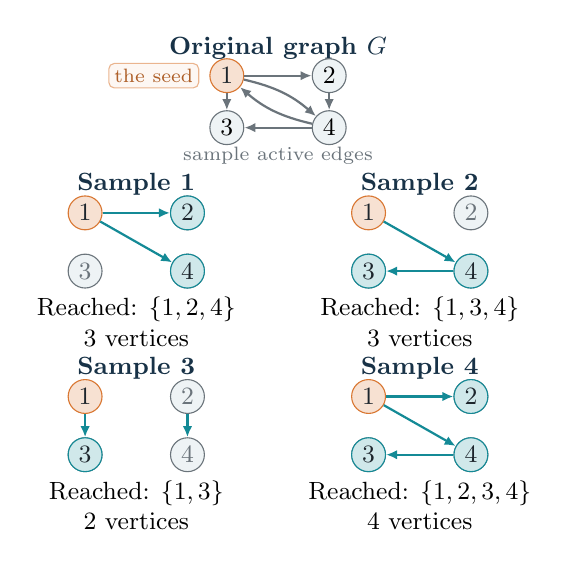
\begin{tikzpicture}[x=1cm,y=0.88cm,>={Latex[length=1.4mm,width=1.2mm]},
  vertex/.style={circle,draw=MidGray,fill=Mist,minimum size=0.43cm,inner sep=0pt,font=\small},
  source/.style={vertex,draw=Orange,fill=Orange!22,text=Ink},
  reached/.style={vertex,draw=Teal,fill=Teal!20,text=Ink},
  every node/.style={font=\small,align=center}]
  \node[font=\small\bfseries,text=DeepNavy] at (2.8,0) {Original graph $G$};
  \node[source] (g1) at (2.15,-0.4) {1};
  \node[anchor=east,font=\scriptsize,text=Orange!80!black,
    draw=Orange!55,fill=Orange!6,rounded corners=2pt,inner sep=2pt]
    at (1.8,-0.4) {the seed};
  \node[vertex] (g2) at (3.45,-0.4) {2};
  \node[vertex] (g3) at (2.15,-1.15) {3};
  \node[vertex] (g4) at (3.45,-1.15) {4};
  \draw[->,thick,MidGray] (g1)--(g2);
  \draw[->,thick,MidGray] (g1)--(g3);
  \draw[->,thick,MidGray] (g2)--(g4);
  \draw[->,thick,MidGray] (g4)--(g3);
  \draw[->,thick,MidGray] (g1) to[bend left=14] (g4);
  \draw[->,thick,MidGray] (g4) to[bend left=14] (g1);
  \node[font=\scriptsize,text=MidGray] at (2.8,-1.55) {sample active edges};
  % Same four sampled edge sets as the layered view on slide 7.
  \foreach \offset/\base/\sample in {0/0/1,3.6/0/2,0/-2.65/3,3.6/-2.65/4}{
    \begin{scope}[xshift=\offset cm,yshift=\base*0.88 cm]
      \node[font=\small\bfseries,text=DeepNavy] at (1,-1.97) {Sample \sample};
      \node[source] (a\sample) at (0.35,-2.38) {1};
      \node[vertex,text=MidGray] (b\sample) at (1.65,-2.38) {2};
      \node[vertex,text=MidGray] (c\sample) at (0.35,-3.22) {3};
      \node[vertex,text=MidGray] (d\sample) at (1.65,-3.22) {4};
    \end{scope}
  }
  \node[reached] at (b1) {2};
  \node[reached] at (d1) {4};
  \node[reached] at (c2) {3};
  \node[reached] at (d2) {4};
  \node[reached] at (c3) {3};
  \node[reached] at (b4) {2};
  \node[reached] at (c4) {3};
  \node[reached] at (d4) {4};
  \draw[->,thick,Teal] (a1)--(b1);
  \draw[->,thick,Teal] (a1)--(d1);
  \draw[->,thick,Teal] (a2)--(d2);
  \draw[->,thick,Teal] (d2)--(c2);
  \draw[->,thick,Teal] (a3)--(c3);
  \draw[->,thick,Teal] (b3)--(d3);
  \draw[->,thick,Teal] (a4)--(b4);
  \draw[->,thick,Teal] (a4)--(d4);
  \draw[->,thick,Teal] (d4)--(c4);
  \node at (1,-3.95) {Reached: $\{1,2,4\}$\\3 vertices};
  \node at (4.6,-3.95) {Reached: $\{1,3,4\}$\\3 vertices};
  \node at (1,-6.60) {Reached: $\{1,3\}$\\2 vertices};
  \node at (4.6,-6.60) {Reached: $\{1,2,3,4\}$\\4 vertices};
\end{tikzpicture}
\end{columns}
\end{frame}

\note{\small\textbf{Slide 6: 80 seconds; finish at 5:05.} Guide attention from the objective to the graph example. Each edge succeeds independently with its given probability. The four samples reach three, three, two, and four vertices, including the source. Sample 3 retains edge 2 to 4, but neither endpoint is reachable from source 1. These are the same four samples shown on the next slide. After explaining the samples, point to the expanded teal simulation loop. Its Reach formula defines the vertices reachable from the trial seed set S; the average below the loop estimates expected reach. Walk through edge sampling, visited state, frontier termination, and distinct-vertex counting. The optimizer uses differences of reach estimates to score additions to the seed set. The gray outer block only supplies optimization context. End with repeated topology access across candidates and simulations.}

% MAIN 07 | 60 seconds | cumulative 6:05
\begin{frame}{Where is the regularity hiding?}
\relax
\begin{columns}[T,onlytextwidth]
\column{0.48\textwidth}
\centering\textbf{The same graph across samples}\par
\vspace{0.05cm}
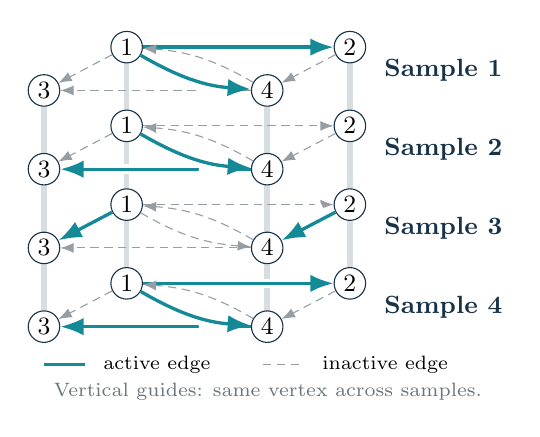
\begin{tikzpicture}[x=1.05cm,y=1cm,>=Latex,
  vertex/.style={circle,draw=DeepNavy,fill=white,minimum size=0.4cm,inner sep=0pt,font=\small},
  active/.style={->,very thick,Teal,preaction={draw=white,line width=3.5pt}},
  inactive/.style={->,densely dashed,MidGray!70,thin},
  every node/.style={font=\small}]
  % Four sample layers correspond to the four-lane example on the next slide.
  \foreach \v/\x/\y in {1/1/0.55,2/3.7/0.55,3/0/0,4/2.7/0}{
    \draw[LightGray,line width=2pt] (\x,\y)--(\x,\y+3);
  }
  \foreach \layer/\base in {1/3,2/2,3/1,4/0}{
    \begin{scope}[yshift=\base cm]
      \node[vertex] (s\layer1) at (1,0.55) {1};
      \node[vertex] (s\layer2) at (3.7,0.55) {2};
      \node[vertex] (s\layer3) at (0,0) {3};
      \node[vertex] (s\layer4) at (2.7,0) {4};
      \node[anchor=west,font=\small\bfseries,text=DeepNavy] at (4,0.25) {Sample \layer};
    \end{scope}
  }
  \draw[active] (s11) -- (s12);
  \draw[inactive] (s11) -- (s13);
  \draw[inactive] (s12) -- (s14);
  \draw[inactive] (s14) -- (s13);
  \draw[active] (s11) to[bend right=13] (s14);
  \draw[inactive] (s14) to[bend right=13] (s11);
  \draw[inactive] (s21) -- (s22);
  \draw[inactive] (s21) -- (s23);
  \draw[inactive] (s22) -- (s24);
  \draw[active] (s24) -- (s23);
  \draw[active] (s21) to[bend right=13] (s24);
  \draw[inactive] (s24) to[bend right=13] (s21);
  \draw[inactive] (s31) -- (s32);
  \draw[active] (s31) -- (s33);
  \draw[active] (s32) -- (s34);
  \draw[inactive] (s34) -- (s33);
  \draw[inactive] (s31) to[bend right=13] (s34);
  \draw[inactive] (s34) to[bend right=13] (s31);
  \draw[active] (s41) -- (s42);
  \draw[inactive] (s41) -- (s43);
  \draw[inactive] (s42) -- (s44);
  \draw[active] (s44) -- (s43);
  \draw[active] (s41) to[bend right=13] (s44);
  \draw[inactive] (s44) to[bend right=13] (s41);
  \draw[Teal,very thick] (0,-0.48)--(0.5,-0.48);
  \node[anchor=west,font=\scriptsize] at (0.6,-0.48) {active edge};
  \draw[MidGray!70,densely dashed] (2.65,-0.48)--(3.15,-0.48);
  \node[anchor=west,font=\scriptsize] at (3.25,-0.48) {inactive edge};
  \node[anchor=west,font=\scriptsize,text=MidGray] at (0,-0.82)
    {Vertical guides: same vertex across samples.};
\end{tikzpicture}
\column{0.48\textwidth}
\centering\textbf{One topology, sample membership on edges}\par
\vspace{0.1cm}
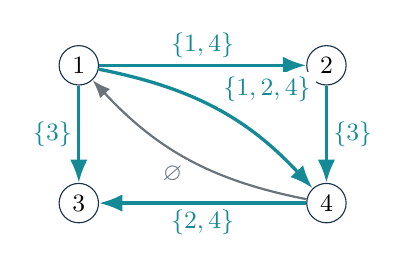
\begin{tikzpicture}[x=0.85cm,y=0.7cm,>=Latex,
  vertex/.style={circle,draw=DeepNavy,fill=white,minimum size=0.5cm,inner sep=0pt,font=\small},
  membership/.style={font=\small,fill=white,inner sep=2pt},
  every node/.style={font=\small}]
  \node[vertex] (g1) at (0.7,3) {1};
  \node[vertex] (g2) at (4.4,3) {2};
  \node[vertex] (g3) at (0.7,0.5) {3};
  \node[vertex] (g4) at (4.4,0.5) {4};
  \draw[->,very thick,Teal] (g1)--node[membership,above] {$\{1,4\}$} (g2);
  \draw[->,very thick,Teal] (g1)--node[membership,left] {$\{3\}$} (g3);
  \draw[->,very thick,Teal] (g2)--node[membership,right] {$\{3\}$} (g4);
  \draw[->,very thick,Teal] (g4)--node[membership,below] {$\{2,4\}$} (g3);
  \draw[->,very thick,Teal] (g1) to[bend left=18]
    node[membership,above right] {$\{1,2,4\}$} (g4);
  \draw[->,thick,MidGray] (g4) to[bend left=18]
    node[membership,below left] {$\varnothing$} (g1);
\end{tikzpicture}
\par
\raggedright
\begin{block}{Shared across samples}
  \small topology · vertices · edges · algorithmic structure
\end{block}
\begin{block}{Changes across samples}
  \small edge membership · active state · random decisions
\end{block}
\end{columns}
\takeaway{Regularity comes from applying the same edge operation across samples.}
\end{frame}

\note{\small\textbf{Slide 7: 60 seconds; finish at 6:05.} Use the bunkbed picture as personal motivation for expecting overlapping edge activity. Trace edge 1 to 4: active in samples 1, 2, and 4, absent from 3. Pause to connect the layers to the membership set. Hold the edge fixed; map four samples to four lanes. Keep separate state and mask inactive work. Distinguish topology reuse from the later scheduling opportunity. Vertical guides indicate vertex identity.}

% MAIN 08 | 145 seconds | cumulative 8:30
\begin{frame}{Parallel lanes across samples}
\setlength{\parskip}{0pt}
{\small\textbf{Vertex-major storage:} each row holds the sample states for one vertex.\par}
\vspace{0.05cm}
\begin{columns}[T,onlytextwidth]
\column{0.48\textwidth}
\setlength{\parskip}{0pt}
\centering\textbf{One sample; parallel neighbors}\par
\par\vspace{0.03cm}
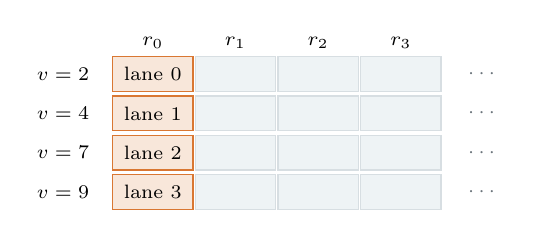
\begin{tikzpicture}[x=1.05cm,y=0.50cm,every node/.style={font=\scriptsize}]
  \foreach \c in {0,...,3}{\node at (\c,0.80) {$r_\c$};}
  \foreach \r/\v in {0/2,1/4,2/7,3/9}{
    \node[anchor=east] at (-0.65,-\r) {$v=\v$};
    \node[text=MidGray] at (4,-\r) {$\cdots$};
    \foreach \c in {0,...,3}{
      \ifnum\c=0
        \node[draw=Orange,fill=Orange!18,minimum width=1.02cm,minimum height=0.44cm] at (\c,-\r) {lane \r};
      \else
        \node[draw=LightGray,fill=Mist,minimum width=1.02cm,minimum height=0.44cm] at (\c,-\r) {};
      \fi
    }
  }
\end{tikzpicture}
\par\vspace{0.05cm}
{\small\textcolor{Orange}{Different rows; scattered state accesses}\par}
\vspace{0.03cm}
{\small\raggedright
\textbf{4 random reads}; likely 4 random writes\par
CPU: non-vector compute\par
GPU: warp/workgroup divergence and stalls\par
{\scriptsize Independent thread scheduling helps;\\
scattered memory access remains expensive.\par}}
\column{0.48\textwidth}
\setlength{\parskip}{0pt}
\centering\textbf{One edge; parallel samples}\par
\par\vspace{0.03cm}
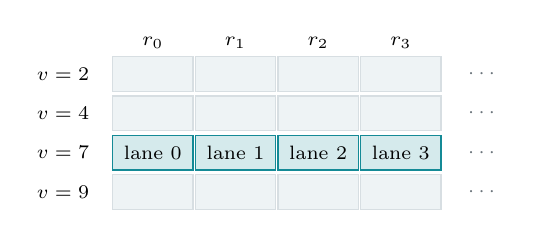
\begin{tikzpicture}[x=1.05cm,y=0.50cm,every node/.style={font=\scriptsize}]
  \foreach \c in {0,...,3}{\node at (\c,0.80) {$r_\c$};}
  \foreach \r/\v in {0/2,1/4,2/7,3/9}{
    \node[anchor=east] at (-0.65,-\r) {$v=\v$};
    \node[text=MidGray] at (4,-\r) {$\cdots$};
    \foreach \c in {0,...,3}{
      \ifnum\r=2
        \node[draw=Teal,fill=Teal!18,minimum width=1.02cm,minimum height=0.44cm] at (\c,-\r) {lane \c};
      \else
        \node[draw=LightGray,fill=Mist,minimum width=1.02cm,minimum height=0.44cm] at (\c,-\r) {};
      \fi
    }
  }
\end{tikzpicture}
\par\vspace{0.05cm}
{\small\textcolor{Teal}{Same row; contiguous state accesses}\par}
\vspace{0.03cm}
{\small\raggedright
\textbf{1 sequential read}; 1 sequential write\par
CPU: vector instructions\par
{\scriptsize ($\sim$2$\times$ latency, $>4\times$ throughput)}\par
GPU: no divergence in the masked update\par
Contributing work varies across lanes\par}
\end{columns}
\par\vspace{0.03cm}
\smallsource{NVIDIA: 32-lane warps. AMD RDNA 3/4: 32/64-lane waves + VLIW-like dual issue.\\
AVX-512: 512 bits ($16\times32$). Arm SVE2: up to 2048 bits ($64\times32$); width depends on the processor.\par}
\end{frame}

\note{\small\textbf{Slide 8: 145 seconds; finish at 8:30.} The highlighted cells show one group of four lanes. On the left, all four lanes work on sample zero, but each follows a different neighbor. On the right, I hold the edge to vertex seven fixed. Compare four random reads and likely four random writes on the left with one sequential read and one sequential write on the right. These describe the logical access pattern, not a universal count of hardware transactions. The left uses non-vector CPU compute and exposes GPU warp/workgroup divergence and stalls. Independent thread scheduling helps with divergent execution, but it does not make scattered memory accesses contiguous; their cost remains high. The right uses CPU vector instructions and a masked GPU update with shared control flow, so it avoids branch divergence within that update. Contributing work still varies across sample lanes. The shaded pattern explains the loop organization. There is an algorithmic constraint. Larger batches can improve reuse but increase state footprint and inactive work.}

% MAIN 09 | 75 seconds | cumulative 9:45
\begin{frame}{Random decisions tied to identity}
\setlength{\parskip}{0pt}
We changed the execution order.\par
\textbf{How do we preserve the same sampled graphs?}\par
\vspace{0.40cm}
\centering
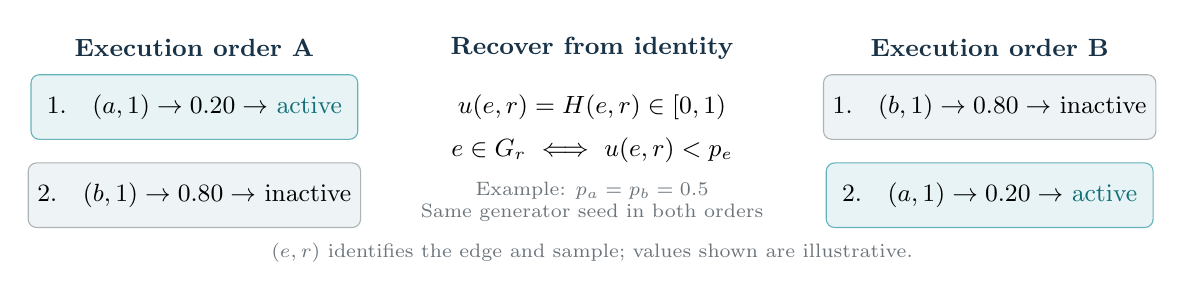
\begin{tikzpicture}[x=1cm,y=1cm,>=Latex,
  every node/.style={font=\small,align=center},
  active/.style={draw=Teal!65,fill=Teal!10,rounded corners=3pt,
    minimum width=4.15cm,minimum height=0.82cm},
  inactive/.style={draw=MidGray!55,fill=Mist,rounded corners=3pt,
    minimum width=4.15cm,minimum height=0.82cm}]
  \node[font=\small\bfseries,text=DeepNavy] at (2.1,0.2) {Execution order A};
  \node[font=\small\bfseries,text=DeepNavy] at (7.15,0.2) {Recover from identity};
  \node[font=\small\bfseries,text=DeepNavy] at (12.2,0.2) {Execution order B};
  \node[active] at (2.1,-0.55) {1.\quad $(a,1)\to 0.20\to$ \textcolor{Teal!80!black}{active}};
  \node[inactive] at (2.1,-1.67) {2.\quad $(b,1)\to 0.80\to$ inactive};
  \node[inactive] at (12.2,-0.55) {1.\quad $(b,1)\to 0.80\to$ inactive};
  \node[active] at (12.2,-1.67) {2.\quad $(a,1)\to 0.20\to$ \textcolor{Teal!80!black}{active}};
  \node at (7.15,-0.55) {$u(e,r)=H(e,r)\in[0,1)$};
  \node at (7.15,-1.10) {$e\in G_r\ \Longleftrightarrow\ u(e,r)<p_e$};
  \node[font=\scriptsize,text=MidGray] at (7.15,-1.75)
    {Example: $p_a=p_b=0.5$\\Same generator seed in both orders};
  \node[font=\scriptsize,text=MidGray] at (7.15,-2.40)
    {$(e,r)$ identifies the edge and sample; values shown are illustrative.};
\end{tikzpicture}
\par\vspace{0.15cm}
\takeaway{Reconstruct edge membership when needed, without storing each sampled graph.}
\end{frame}

\note{\small\textbf{Slide 9: 75 seconds; finish at 9:45.} Connect to slide 8: we changed execution order, so we must preserve each realized sampled graph. An ordinary random stream associates successive draws with execution order; reordering can change the realized graph even if the overall distribution remains valid. In the example, both edge probabilities are 0.5. Identity (a,1) recovers 0.20 and remains active; (b,1) recovers 0.80 and remains inactive, whichever is visited first. Values are illustrative, with a fixed generator seed. I made stochastic decisions recoverable so that execution order became a systems design choice. H denotes a pseudorandom mapping to the unit interval; repeatability alone does not establish the required joint sampling distribution. End with reconstructing rather than storing sampled graphs, leading into compute more, move less.}

% MAIN 10 | 75 seconds | cumulative 11:00
\begin{frame}{Compute more, move less}
\relax
\begin{columns}[T,onlytextwidth]
\column{0.49\textwidth}
\textbf{Additional work}\par
Reconstruct decisions\par
Compare probabilities\par
Mask inactive sample lanes
\par\vspace{0.5cm}
\textbf{Avoided work}\par
Materializing sampled graphs\par
Repeated access to shared topology
\column{0.45\textwidth}
{\Huge\bfseries\color{Teal}$\sim$3--21$\times$\par}
\par\vspace{0.3cm}
Reported contribution of fused sampling\par
\par\vspace{0.3cm}
Sequential \textsc{FusedSampling} vs. \textsc{MixGreedy}; the three graphs where the reference completed.
\end{columns}
\par\vspace{0.5cm}
\takeaway{Instruction count can increase while runtime decreases.}
\smallsource{InFuseR-MG, Table 4 and accompanying discussion; $K=50$. On-the-fly sampling only: samples still run separately; batching and memoization are additional changes.}
\end{frame}

\note{\small\textbf{Slide 10: 75 seconds; finish at 11:00.} We deliberately add hashing, comparisons, and masking. The first paper reports roughly three to twenty-one times improvement from fused sampling in the sequential comparison against MixGreedy, on the three graphs where that reference completed. This particular variant generates decisions on the fly but still processes samples separately. The broader principle is compute more, move less.}

% MAIN 11 | 45 seconds | cumulative 11:45
\begin{frame}{The next bottleneck: per-sample state}
\relax
\begin{columns}[T,onlytextwidth]
\column{0.44\textwidth}
\begin{center}
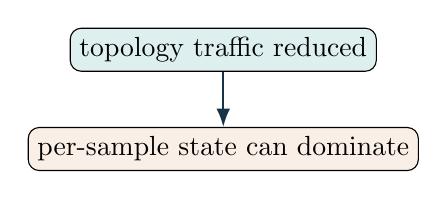
\begin{tikzpicture}[node distance=0.7cm,>=Latex]
  \node[draw,rounded corners,fill=Teal!14,minimum width=3.4cm] (topo) {topology traffic reduced};
  \node[draw,rounded corners,fill=Orange!12,minimum width=3.4cm,below=of topo] (state) {per-sample state can dominate};
  \draw[->,thick,DeepNavy] (topo)--(state);
\end{tikzpicture}
\end{center}
\par\vspace{0.6em}
Even one exact label per vertex per sample requires:
\[
\text{label storage}=\Theta(|V|R)
\]

\column{0.52\textwidth}
\textbf{What does the downstream computation actually need?}
\begin{itemize}
  \item exact reached set?
  \item only its cardinality?
\end{itemize}
\par\vspace{0.5em}
\emphbox{From regularity across samples to uniform state and updates.}
\end{columns}
\takeaway{Preserve the information the query needs -- not necessarily every intermediate state.}
\end{frame}

\note{\small\textbf{Slide 11: 45 seconds; finish at 11:45.} So far, we found regularity across samples. Next, change the representation so that state and updates become more uniform. Sharing topology does not eliminate sample state. Ask what the downstream query needs; compact summaries introduce an accuracy tradeoff.}

% MAIN 12 | 130 seconds | cumulative 13:55
\begin{frame}{Compact representations, uniform updates}
\relax
\begin{columns}[T,onlytextwidth]
\column{0.48\textwidth}
\textbf{Query}\par
How many distinct vertices are reachable?
\par\vspace{0.35cm}
\textbf{Count-distinct summary}\par
Hash vertex identities; retain a small register summarizing rare bit patterns.
\column{0.48\textwidth}
\textbf{Merge through an active edge}\par
\[
M_u[j]\gets\max\bigl(M_u[j],M_v[j]\bigr)
\]
Fixed-width registers across samples\par
Contiguous loads and vector maximum
\end{columns}
\par\vspace{0.45cm}
\textbf{Why it works:} repeated paths do not double-count a vertex; merging the same summary again leaves it unchanged.
\par\vspace{0.2cm}
\takeaway{Retain a cardinality estimate instead of materializing every reached set.}
\smallsource{HyperFuseR, Secs. 2.2 and 3. One small register per vertex per sample; approximation and error-adaptive rebuilding remain part of the method.}
\end{frame}

\note{\small\textbf{Slide 12: 130 seconds; finish at 13:55.} HyperFuseR uses a compact count-distinct summary. The crucial operation is merge. In this algorithm, a register position is associated with a stochastic sample, and propagation is gated by that sample's edge decisions. There is a price: sketch error and decisions about rebuilding the summaries as the selected source set changes. The architectural result is compact, contiguous state with a cheap merge.}

% MAIN 13 | 60 seconds | cumulative 14:55
\begin{frame}{Mapping the sample dimension to hardware}
\relax
\emphbox{The regular sample dimension stays the same; the low-level mapping changes.}
\par\vspace{0.55em}
\begin{columns}[T,onlytextwidth]
\column{0.31\textwidth}
\begin{block}{CPU}
\centering\textbf{SIMD lanes}\\[0.45em]
{\small contiguous vector state\\cache reuse · masked lanes}
\end{block}
\column{0.31\textwidth}
\begin{block}{GPU}
\centering\textbf{Warp threads}\\[0.45em]
{\small nearby sample-state accesses\\similar work within a warp}
\end{block}
\column{0.31\textwidth}
\begin{block}{Multiple GPUs}
\centering\textbf{Sample partitions}\\[0.45em]
{\small local propagation\\edge overlap · global reduction}
\end{block}
\end{columns}
\par\vspace{0.5em}
\begin{center}
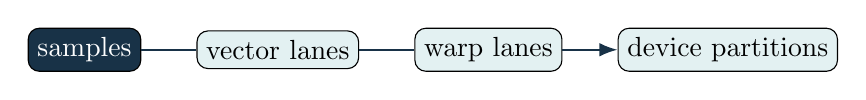
\begin{tikzpicture}[>=Latex,node distance=0.7cm]
  \node[draw,rounded corners,fill=DeepNavy,text=white] (s) {samples};
  \node[draw,rounded corners,fill=Teal!12,right=of s] (v) {vector lanes};
  \node[draw,rounded corners,fill=Teal!12,right=of v] (w) {warp lanes};
  \node[draw,rounded corners,fill=Teal!12,right=of w] (d) {device partitions};
  \draw[->,thick,DeepNavy] (s)--(v)--(w)--(d);
\end{tikzpicture}
\end{center}
\takeaway{The abstraction is portable; the mapping is architecture-specific.}
\smallsource{Research progression: InFuseR-MG $\rightarrow$ HyperFuseR $\rightarrow$ DiFuseR.}
\end{frame}

\note{\small\textbf{Slide 13: 60 seconds; finish at 14:55.} The sample dimension survives across architectures. Across GPUs, I partition samples. The abstraction is portable, while batch sizes, scheduling, and communication remain architecture-specific.}

% MAIN 14 | 100 seconds | cumulative 16:35
\begin{frame}{FASST: sample order changes hardware utilization}
\relax
\begin{columns}[T,onlytextwidth]
\column{0.49\textwidth}
\centering\textbf{Naïve assignment}\par\vspace{0.45em}
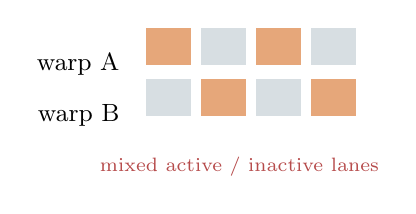
\begin{tikzpicture}[x=0.7cm,y=0.65cm]
  \foreach \r in {0,1}{
    \node[anchor=east,font=\small] at (-0.3,-\r) {warp \ifnum\r=0 A\else B\fi};
    \foreach \c in {0,...,3}{
      \pgfmathtruncatemacro{\z}{mod(\c+\r,2)}
      \ifnum\z=0 \def\cc{Orange!65}\else\def\cc{LightGray}\fi
      \fill[\cc] (\c,-\r) rectangle ++(0.82,0.72);
    }
  }
  \node[font=\scriptsize\color{SoftRed}] at (1.7,-2.0) {mixed active / inactive lanes};
\end{tikzpicture}

\column{0.47\textwidth}
\centering\textbf{Sampling-aware assignment}\par\vspace{0.45em}
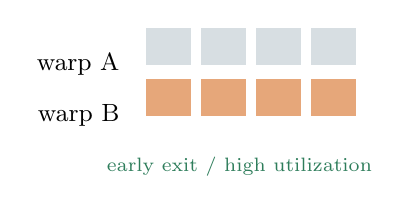
\begin{tikzpicture}[x=0.7cm,y=0.65cm]
  \node[anchor=east,font=\small] at (-0.3,0) {warp A};
  \node[anchor=east,font=\small] at (-0.3,-1) {warp B};
  \foreach \c in {0,...,3}{
    \fill[LightGray] (\c,0) rectangle ++(0.82,0.72);
    \fill[Orange!65] (\c,-1) rectangle ++(0.82,0.72);
  }
  \node[font=\scriptsize\color{Success}] at (1.7,-2.0) {early exit / high utilization};
\end{tikzpicture}
\end{columns}
\par\vspace{0.7em}
FASST sorts the existing sample keys, then assigns nearby keys to warps and device partitions. For a fixed edge, related decisions can cluster.
\takeaway{A whole inactive warp can skip an edge; a device can omit edges unused by its samples.}
\smallsource{DiFuseR, Sec. 4.1. Schematic for one edge; perfect grouping is not guaranteed for every edge.}
\end{frame}

\note{\small\textbf{Slide 14: 100 seconds; finish at 16:35.} Mapping samples to lanes exposes another degree of freedom: which samples should be neighbors? In the left-hand schematic, each warp contains a mixture of samples where this edge is active and inactive. FASST sorts the existing sample keys before assigning them to warps and devices. The same grouping matters at device scale. The estimator averages over the same sample identities.}

% MAIN 15 | 60 seconds | cumulative 17:35
\begin{frame}{Sample-space decomposition scales across GPUs}
\relax
\begin{columns}[c,onlytextwidth]
\column{0.46\textwidth}
\centering
\renewcommand{\arraystretch}{1.3}
\begin{tabular}{@{}rr@{}}
\toprule
\textbf{A100 GPUs} & \textbf{Speedup vs. 1 GPU}\\
\midrule
1 & 1.00$\times$\\
2 & 2.45$\times$\\
4 & 4.28$\times$\\
8 & \textcolor{Teal}{\bfseries 5.64$\times$}\\
\bottomrule
\end{tabular}
\column{0.49\textwidth}
\textbf{Local work}\par
Propagate sketches over each device's samples and required edges.
\par\vspace{0.4cm}
\textbf{Global work}\par
Reduce local estimates to select the next source.
\end{columns}
\par\vspace{0.4cm}
\takeaway{The sample dimension provides a distributed decomposition with useful locality.}
\smallsource{DiFuseR, Table 8: geometric means, $K=50$, $J=1024$; two GPUs per node for multi-GPU runs. Friendster excluded because the one-GPU configuration does not fit.}
\end{frame}

\note{\small\textbf{Slide 15: 60 seconds; finish at 17:35.} Here is the distributed evidence I want to emphasize. This is useful scaling, not perfect scaling. The architectural lesson is that stochastic samples are a useful unit of distributed decomposition.}

% MAIN 16 | 75 seconds | cumulative 18:50
\begin{frame}{A harder case: random walks destroy exact alignment}
\relax
\begin{columns}[T,onlytextwidth]
\column{0.45\textwidth}
A random walk is sequential within a trajectory:
\begin{center}
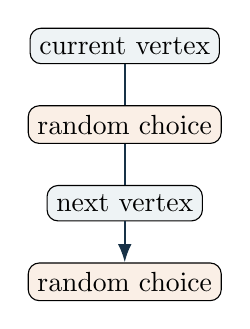
\begin{tikzpicture}[node distance=0.52cm,>=Latex]
  \node[draw,rounded corners,fill=Mist] (a) {current vertex};
  \node[draw,rounded corners,fill=Orange!12,below=of a] (b) {random choice};
  \node[draw,rounded corners,fill=Mist,below=of b] (c) {next vertex};
  \node[draw,rounded corners,fill=Orange!12,below=of c] (d) {random choice};
  \draw[->,thick,DeepNavy] (a)--(b)--(c)--(d);
\end{tikzpicture}
\end{center}

\column{0.51\textwidth}
\begin{center}
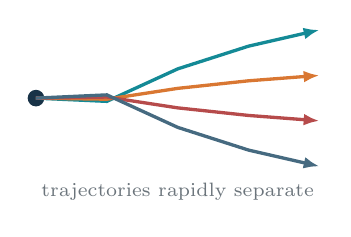
\begin{tikzpicture}[x=0.9cm,y=0.55cm,>=Latex]
  \coordinate (s) at (0,0);
  \fill[DeepNavy] (s) circle (3pt);
  \foreach \i/\ang/\cc in {0/25/Teal,1/5/Orange,2/-18/SoftRed,3/-35/Steel}{
    \draw[-{Latex[length=2mm]},\cc,very thick] (0,0) -- (1, {0.05*(\i-1.5)}) -- (2,{0.45*(1.5-\i)}) -- (3,{0.8*(1.5-\i)}) -- (4,{1.05*(1.5-\i)});
  }
  \node[font=\scriptsize\color{MidGray}] at (2,-2.15) {trajectories rapidly separate};
\end{tikzpicture}
\end{center}
\begin{itemize}
  \item next address depends on previous random choice
  \item exact lane alignment disappears quickly
\end{itemize}
\end{columns}
\takeaway{Now we need a scheduling method, not just a different loop order.}
\end{frame}

\note{\small\textbf{Slide 16: 75 seconds; finish at 18:50.} A random walk takes us into a harder regime. In the earlier algorithms, I could hold a graph edge fixed and process many samples against it. Assigning one walk to each vector lane exposes parallel work but may also expose many unrelated cache misses at once.}

% MAIN 17 | 135 seconds | cumulative 21:05
\begin{frame}{SABA: seed ordering creates opportunities for reuse}
\relax
First step from $s$: four equal-probability neighbors.
\par{\small $[0,.25)\to A\quad [.25,.50)\to B\quad [.50,.75)\to C\quad [.75,1)\to D$}\par\vspace{0.12cm}
\begin{columns}[T,onlytextwidth]
\column{0.48\textwidth}
\centering\textbf{Unordered groups of four}\par\vspace{0.15cm}
\renewcommand{\arraystretch}{1.10}
\begin{tabular}{@{}lcccc@{}}
seeds & .83 & .14 & .63 & .29\\
next vertex & $D$ & $A$ & $C$ & $B$\\[0.35em]
seeds & .91 & .48 & .05 & .72\\
next vertex & $D$ & $B$ & $A$ & $C$\\
\end{tabular}
\par\vspace{0.2cm}
\textcolor{Orange}{4 distinct adjacency rows per group}
\column{0.48\textwidth}
\centering\textbf{Sorted groups of four}\par\vspace{0.15cm}
\renewcommand{\arraystretch}{1.10}
\begin{tabular}{@{}lcccc@{}}
seeds & .05 & .14 & .29 & .48\\
next vertex & \textcolor{Teal}{$A$} & \textcolor{Teal}{$A$} & $B$ & $B$\\[0.35em]
seeds & .63 & .72 & .83 & .91\\
next vertex & \textcolor{Teal}{$C$} & \textcolor{Teal}{$C$} & $D$ & $D$\\
\end{tabular}
\par\vspace{0.2cm}
\textcolor{Teal}{2 distinct adjacency rows per group}
\end{columns}
\par\vspace{0.1cm}
\takeaway{Nearby seeds reuse early adjacency; walks can diverge at the next step.}
\smallsource{Toy example with normalized, independently drawn seeds; not measured data.}
\end{frame}

\note{\small\textbf{Slide 17: 135 seconds; finish at 21:05.} Here is what sorting actually changes. In the first unordered group, the seeds choose D, A, C, and B. That is the locality opportunity. Exact alignment need not persist. The method therefore uses statistical structure to improve a schedule, rather than requiring every lane to follow the same path. The remaining question is whether the same construction can give valid multi-step walks.}

% MAIN 18 | 90 seconds | cumulative 22:35
\begin{frame}{Correct sampling and useful grouping}
\relax
At a vertex with $d$ neighbors:\quad $x\sim\mathrm{Uniform}\{0,\ldots,R-1\}$
\[
q=\lfloor R/d\rfloor,\qquad
k=\lfloor x/q\rfloor,\qquad
x' = x\bmod q,\quad R'=q
\]
\centering
\begin{tabular}{@{}lccc@{}}
\toprule
Example: $R=12$, $d=3$ & $x=0,\ldots,3$ & $x=4,\ldots,7$ & $x=8,\ldots,11$\\
\midrule
Chosen neighbor $k$ & 0 & 1 & 2\\
Retained residual $x'$ & $0,1,2,3$ & $0,1,2,3$ & $0,1,2,3$\\
\bottomrule
\end{tabular}
\par\vspace{0.3cm}\raggedright
If $q=0$ or $x\ge dq$: switch permanently to fresh, unbiased conventional sampling.
\par\vspace{0.2cm}
\takeaway{Uniform next choice given the path history; unused randomness retained for later steps.}
\smallsource{Revised SABA manuscript, Sec. 3.2. Assumes ideal independent random inputs. Reordering a fixed set of valid walks is a separate estimator invariance.}
\end{frame}

\note{\small\textbf{Slide 18: 90 seconds; finish at 22:35.} The requirement is conditional: given the path so far, the next choice must be uniform over the current neighbors. In this small integer example, x is uniform over twelve values and the current vertex has three neighbors. Each neighbor has four possible inputs. When the residual is too small or falls in a rejected remainder, the walk permanently switches to fresh unbiased conventional sampling. This is the sampler-validity argument.}

% MAIN 19 | 60 seconds | cumulative 23:35
\begin{frame}{Parallelism without locality can increase cache misses}
\relax
\begin{columns}[T,onlytextwidth]
\column{0.52\textwidth}
\renewcommand{\arraystretch}{1.22}
\begin{tabular}{@{}lr@{}}
\toprule
\textbf{Reported method} & \textbf{L3 misses / naïve}\\
\midrule
Naïve scalar walks & 100.00\%\\
Direct AVX2 & \textcolor{SoftRed}{\bfseries 108.83\%}\\
HASH vector baseline & 61.92\%\\
SABA ordering & \textcolor{Teal}{\bfseries 3.55\%}\\
\bottomrule
\end{tabular}
\column{0.44\textwidth}
\textbf{Architectural observation}\par
More vector execution did not ensure fewer cache misses.
\par\vspace{0.3cm}
\textbf{Reported ordering comparison}\par
3.38$\times$ walk-processing speedup over HASH at 16,384 walks/vertex.
\end{columns}
\par\vspace{0.25cm}
\takeaway{Useful parallel execution depends on locality as well as arithmetic throughput.}
\par\vspace{0.15cm}
{\small\textbf{Scope:} historical sampler measurements; these tables do not validate the corrected residual-range method.}
\smallsource{SABA manuscript, Sec. 5 validation status and Tables 5, 7. Cache ratios: geometric means over 10 graphs, 16,384 walks/vertex; Broadwell Xeons. Runtime comparison uses 16 threads.}
\end{frame}

\note{\small\textbf{Slide 19: 60 seconds; finish at 23:35.} The reported measurements illustrate why we must inspect memory behavior. These tables describe the earlier sampler and do not validate the corrected residual-range version. The systems lesson is that vectorization and locality are distinct.}

% MAIN 20 | 50 seconds | cumulative 24:25
\begin{frame}{A methodology for irregular computation}
\relax
\renewcommand{\arraystretch}{1.2}
\begin{tabular}{@{}>{\raggedright\arraybackslash}p{3.1cm}>{\raggedright\arraybackslash}p{7.0cm}>{\raggedright\arraybackslash}p{2.7cm}@{}}
\toprule
\textbf{Obstacle} & \textbf{Research move} & \textbf{Work}\\
\midrule
Repeated topology access & Parallelize across samples; reconstruct decisions & InFuseR-MG\\
Large intermediate state & Retain mergeable cardinality information & HyperFuseR\\
Inactive lanes, edge overlap & Order and partition sample space & DiFuseR / FASST\\
Path-dependent addresses & Group trajectories using sampling structure & SABA\\
\bottomrule
\end{tabular}
\par\vspace{0.4cm}
\takeaway{Identify the bottleneck, expose usable regularity, and preserve the relevant contract.}
\end{frame}

\note{\small\textbf{Slide 20: 50 seconds; finish at 24:25.} The projects connect through the kind of freedom each one uses. The contribution is the connection between an algorithmic choice and the architectural cost it changes.}

% MAIN 21 | 40 seconds | cumulative 25:05
\begin{frame}{When restructuring pays off}
\relax
\begin{columns}[T,onlytextwidth]
\column{0.49\textwidth}
\begin{block}{Favorable conditions}
\begin{itemize}
  \item[\yes] abundant independent work
  \item[\yes] repeatedly visited sparse structure
  \item[\yes] memory-bound execution
  \item[\yes] compact state / useful summaries
  \item[\yes] schedules that create locality or coherence
\end{itemize}
\end{block}

\column{0.49\textwidth}
\begin{block}{Less favorable conditions}
\begin{itemize}
  \item[\no] too little work to fill wide machines
  \item[\no] compute-bound kernels
  \item[\no] long trajectories with little reuse
  \item[\no] state that cannot be compressed
  \item[\no] ordering overhead exceeds saved traffic
\end{itemize}
\end{block}
\end{columns}
\takeaway{Saved memory stalls and idle-lane work must exceed ordering, state, and coordination costs.}
\end{frame}

\note{\small\textbf{Slide 21: 40 seconds; finish at 25:05.} These transformations pay off only when there is enough independent work and enough reusable structure. A wider batch can improve reuse while increasing state footprint.}

% MAIN 22 | 85 seconds | cumulative 26:30
\begin{frame}{Ongoing work: fused walks for graph learning}
\relax
\textbf{NeuralBloom: accelerating NeuralWalker's input construction}\par
\textbf{Reduce data movement:} fuse walk transitions and structural encodings.
\par\vspace{0.2cm}
\begin{columns}[T,onlytextwidth]
\column{0.65\textwidth}
\textbf{Separate tensor operations}
\begin{itemize}
  \item Dispatch work at successive walk positions
  \item Move intermediate state through GPU memory
  \item Construct structural encodings afterward
\end{itemize}
\textbf{Fused GPU execution}\par
One thread advances a walk; private state and encoding construction stay in one kernel.
\column{0.30\textwidth}
\centering\vspace{0.3cm}
{\Huge\bfseries\color{Teal}$\sim$2$\times$\par}
\vspace{0.2cm}
Preliminary speedup\par
in walk computation
\end{columns}
\par\vspace{0.3cm}
\smallsource{Ongoing NeuralBloom work. Preliminary compute result; not an end-to-end training speedup.}
\end{frame}

\note{\small\textbf{Slide 22: 85 seconds; finish at 26:30.} This connection to machine learning is now active work. A direct tensor implementation can dispatch work at successive walk positions and move intermediate state through global memory. My current experiments show roughly a twofold compute speedup. The opportunity is to reduce data movement and dispatch overhead through fusion while preserving the model-facing representation. Sources: NeuralBloom README and paper/main.tex; preliminary speedup supplied by the presenter. Timing scope is walk computation, not complete training.}

% MAIN 23 | 105 seconds | cumulative 28:15
\begin{frame}{Ongoing work: reconstruction and trajectory execution}
\relax
\begin{columns}[T,onlytextwidth]
\column{0.48\textwidth}
\textbf{Battus: diffusion reconstruction}\par
Infer missing graph states between sparse snapshots.
\par\vspace{0.3cm}
\begin{itemize}
  \item Approximate per-vertex probabilities
  \item Forward--backward inference
  \item Regular graph passes mapped to CUDA
\end{itemize}
\par\vspace{0.2cm}
\textbf{Research question}\par
Which inference stages and state are needed for useful reconstruction?
\column{0.48\textwidth}
\textbf{Trajectory-based graph traversal}\par
Represent paths by coordinates that evolve at each step.
\par\vspace{0.3cm}
\begin{itemize}
  \item Deterministic trajectory prototype
  \item Interleave trajectories on the CPU
  \item Map trajectories to GPU threads
\end{itemize}
\par\vspace{0.2cm}
\textbf{Research question}\par
Can interleaving hide memory latency when locality is limited?
\end{columns}
\par\vspace{0.1cm}
\smallsource{Ongoing projects. Battus uses approximate inference; deterministic trajectories are not claimed to be independent Monte Carlo walks.}
\end{frame}

\note{\small\textbf{Slide 23: 105 seconds; finish at 28:15.} Two other ongoing projects explore different algorithmic freedoms. The research question is which inference stages and intermediate state are actually needed for useful reconstruction. The trajectory project explores path coordinates and execution schedules. When locality is limited, interleaving independent trajectories may still overlap memory latency. This extends the broader bottleneck-driven methodology. Together these projects extend the program across execution order, representation, and approximation. Sources: Battus paper/sections/method.tex; randomwalk/walk.h and AGENTS.md. Both are ongoing projects with distinct approximation contracts.}

% MAIN 24 | 115 seconds | cumulative 30:10
\begin{frame}{Finding regularity systematically}
\relax
\textbf{Can we identify useful regularity and decide when exploiting it pays off?}\par
First project: an adaptive trajectory scheduler using observations of reuse and stalls.
\par\vspace{0.35cm}
\renewcommand{\arraystretch}{1.35}
\begin{tabular}{@{}p{2.4cm}>{\raggedright\arraybackslash}p{10.3cm}@{}}
\textbf{Observe} & repeated vertices, active lanes, state footprint, scheduling overhead\\
\textbf{Decide} & keep the order, regroup a batch, or interleave trajectories\\
\textbf{Preserve} & application-defined dependencies, random streams, and accuracy targets\\
\textbf{Deliver} & a runtime policy that reduces total execution time on held-out workloads
\end{tabular}
\par\vspace{0.35cm}
\textbf{First workloads:} graph walks and NeuralBloom.
\end{frame}

\note{\small\textbf{Slide 24: 115 seconds; finish at 30:10.} Can we systematically identify useful regularity and decide when exploiting it is worth the cost? Start with an adaptive trajectory scheduler. Hypothesis: short observations of reuse and stalls predict whether regrouping pays off. Choose current order, regrouping, or interleaving; account for all overhead and preserve dependencies, random-stream ownership, and accuracy. First workloads: graph walks and NeuralBloom.}

% MAIN 25 | 30 seconds | cumulative 30:40
\begin{frame}[plain]{}
\relax
\centering\color{DeepNavy}
{\Large\bfseries Finding Regularity\par}
\par\vspace{0.4cm}
\normalsize
\begin{tabular}{@{}ll@{}}
\textbf{Sample structure} & Share topology across independent samples.\\[0.6em]
\textbf{Compact representations} & Retain useful information; use uniform merges.\\[0.6em]
\textbf{Sampling-aware schedules} & Encourage reuse when trajectories diverge.
\end{tabular}\par
\par\vspace{0.4cm}
\textbf{Next: make these choices systematic, with correctness and cost explicit.}\par
\par\vspace{0.4cm}
\textbf{Questions}
\end{frame}

\note{\small\textbf{Slide 25: 30 seconds; finish at 30:40.} Return to Finding Regularity: sample structure, compact representations, and sampling-aware schedules. The goal is to make these choices systematic while preserving correctness and accounting for total cost.}

\appendix

\begin{frame}[plain,noframenumbering]\centering\Huge\bfseries Backup slides\end{frame}
\relax

\begin{frame}{Backup: fused-sampling implementation in InFuseR-MG}
\relax
For undirected graphs, use a symmetric edge hash:
\[
  h(u,v)=\mathrm{MURMUR3}(\min(u,v)\,\|\,\max(u,v))
\]
so $h(u,v)=h(v,u)$.

For simulation $r$:
\[
  \rho(u,v)_r=\frac{X_r\oplus h(u,v)}{h_{\max}}
\]
and edge $(u,v)$ is active iff
\[
  \rho(u,v)_r\le w_{u,v}.
\]
\takeaway{The system can reconstruct membership from edge/sample identity without materializing sampled graphs.}
\smallsource{InFuseR-MG, Sec. 3.1. Reconstructibility does not by itself prove joint independence across edges.}
\end{frame}

\begin{frame}{Backup: SIMD implementation details}
\relax
\begin{columns}[T,onlytextwidth]
\column{0.55\textwidth}
AVX2 processes eight 32-bit sample states at a time.
\begin{enumerate}
  \item compare component labels
  \item broadcast precomputed edge hash
  \item XOR with simulation seeds
  \item compare against probability threshold
  \item masked / blended updates
  \item movemask-style reduction for changed lanes
\end{enumerate}
\column{0.41\textwidth}
\begin{center}
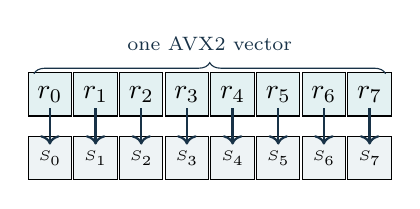
\begin{tikzpicture}[x=0.58cm,y=0.58cm]
  \foreach \i in {0,...,7}{
    \node[draw,fill=Teal!12,minimum size=0.55cm] at (\i,2) {$r_{\i}$};
    \node[draw,fill=Mist,minimum size=0.55cm,font=\tiny] at (\i,0.6) {$S_\i$};
    \draw[->,DeepNavy,thick] (\i,1.7)--(\i,0.9);
  }
  \draw[decorate,decoration={brace,amplitude=4pt},DeepNavy] (-0.35,2.45)--(7.35,2.45) node[midway,above=5pt,font=\scriptsize] {one AVX2 vector};
\end{tikzpicture}
\end{center}
Per-vertex sample state is contiguous, so one vector load fetches several simulations for the same vertex.
\end{columns}
\smallsource{Source: InFuseR-MG, Secs. 3.2--3.3.}
\end{frame}

\begin{frame}{Backup: HyperFuseR sketch details}
\relax
Flajolet--Martin style register update:
\[
M[j]=\max\!\left(M[j],\operatorname{clz}(h_j(x))\right)
\]
Sketch merge:
\[
M_{uv}[j]=\max(M_u[j],M_v[j])
\]
\begin{center}
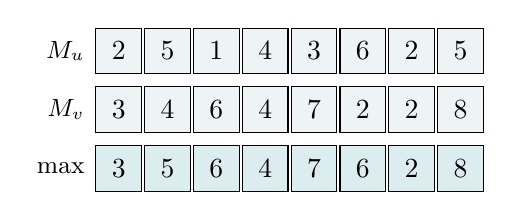
\begin{tikzpicture}[x=0.62cm,y=0.62cm]
  \foreach \i/\a/\b in {0/2/3,1/5/4,2/1/6,3/4/4,4/3/7,5/6/2,6/2/2,7/5/8}{
    \node[draw,fill=Mist,minimum size=0.58cm] at (\i,1.2) {\a};
    \node[draw,fill=Mist,minimum size=0.58cm] at (\i,0) {\b};
    \pgfmathtruncatemacro{\m}{max(\a,\b)}
    \node[draw,fill=Teal!15,minimum size=0.58cm] at (\i,-1.2) {\m};
  }
  \node[anchor=east,font=\small] at (-0.5,1.2) {$M_u$};
  \node[anchor=east,font=\small] at (-0.5,0) {$M_v$};
  \node[anchor=east,font=\small] at (-0.5,-1.2) {$\max$};
\end{tikzpicture}
\end{center}
\takeaway{Compact registers estimate cardinality; they do not preserve exact reached identities.}
\smallsource{Source: HyperFuseR, Sec. 2.2 / Sec. 3.}
\end{frame}

\begin{frame}{Backup: error-adaptive rebuilding in HyperFuseR}
\relax
After selecting more sources, retained sketches can become less useful for estimating marginal reach.
\par\vspace{0.4cm}
\begin{enumerate}
\item Estimate a candidate's marginal gain from compact state.
\item Compare that estimate with a Monte Carlo evaluation.
\item Rebuild when local and global discrepancy criteria trigger.
\end{enumerate}
\par\vspace{0.3cm}
The paper uses local threshold $\epsilon_l=0.3$ and global threshold $\epsilon_g=0.01$ in its experiments.
\takeaway{These empirical rebuilding thresholds are not universal error guarantees.}
\smallsource{HyperFuseR, Algorithm 1 and Sec. 3.2.}
\end{frame}

\begin{frame}{Backup: FASST -- sample-space tasking}
\relax
\begin{columns}[T,onlytextwidth]
\column{0.52\textwidth}
\textbf{Naïve order}
\[
\{1,3\}\quad\{2,0\}\quad\{0,1\}\quad\{2,3\}
\]
\textbf{Sort / cluster sample keys}
\[
\{0,1\}\quad\{0,1\}\quad\{2,3\}\quad\{2,3\}
\]
\par\vspace{0.3em}
Principle: exploit exchangeability of independent samples; change assignment and schedule, not the sample set or estimator.

\column{0.44\textwidth}
On multiple GPUs, each device receives a sample-space partition and derives the local edge set induced by those samples.
\begin{center}
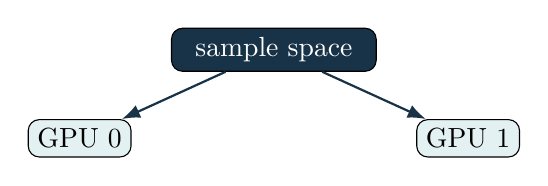
\begin{tikzpicture}[node distance=0.35cm,>=Latex]
  \node[draw,rounded corners,fill=DeepNavy,text=white,minimum width=2.6cm] (s) {sample space};
  \node[draw,rounded corners,fill=Teal!12,below left=0.6cm and 0.5cm of s] (g0) {GPU 0};
  \node[draw,rounded corners,fill=Teal!12,below right=0.6cm and 0.5cm of s] (g1) {GPU 1};
  \draw[->,thick,DeepNavy] (s)--(g0);
  \draw[->,thick,DeepNavy] (s)--(g1);
\end{tikzpicture}
\end{center}
\end{columns}
\smallsource{Source: DiFuseR, Sec. 4.1.}
\end{frame}

\begin{frame}{Backup: multi-GPU scaling}
\relax
\begin{center}
\renewcommand{\arraystretch}{1.25}
\begin{tabular}{@{}r r r@{}}
\toprule
\textbf{GPUs} & \textbf{Observed speedup} & \textbf{Ideal}\\
\midrule
1 & 1.00$\times$ & 1$\times$\\
2 & 2.45$\times$ & 2$\times$\\
4 & 4.28$\times$ & 4$\times$\\
8 & 5.64$\times$ & 8$\times$\\
\bottomrule
\end{tabular}
\end{center}
\par\vspace{1.0em}
\centering
\textbf{Interpretation:} sample-space decomposition exposes a natural distributed axis with limited synchronization; the claim is not perfect scaling.
\par\vspace{0.8em}
\smallsource{DiFuseR, Table 8. Geometric means; $K=50$, $J=1024$; two A100 GPUs per node for multi-GPU runs. Friendster excluded.}
\end{frame}

\begin{frame}{Backup: performance comparisons and their scope}
\relax
\scriptsize
\begin{center}
\begin{tabular}{@{}p{4.1cm} r p{6.1cm}@{}}
\toprule
\textbf{Result} & \textbf{Reported value} & \textbf{What it demonstrates}\\
\midrule
InFuseR-MG vs. state of the art & 2.3--173.8$\times$ & overall effectiveness\\
Fused sampling contribution & $\sim$3--21$\times$ & isolated value of fusing\\
HyperFuseR & up to 119$\times$ & compact-state approach\\
DiFuseR, 1$\times$ A100 & 3.15$\times$ geom. mean vs. gIM & GPU mapping\\
DiFuseR, 8 GPUs & 5.64$\times$ geom. mean vs. 1 GPU & sample-space scale-out\\
Historical SABA, 16,384 walks/vertex & 6.76$\times$ geom. mean vs. naïve & locality-aware vectorized walks\\
Historical SABA vs. matched hash baseline & 3.38$\times$ & scheduling contribution\\
\bottomrule
\end{tabular}
\end{center}
\par\vspace{0.5em}
\begin{alertblock}{Interpretation rule}
SABA rows describe the earlier sampler and do not validate the corrected residual-range method. Other rows compare complete methods unless explicitly identified as fusion or scaling.
\end{alertblock}
\end{frame}

\begin{frame}{Backup: residual-range sampler and unbiased fallback}
\relax
\small
Initial seed: $X_W\sim\mathrm{Uniform}\{0,\ldots,2^{64}-2\}$; set $x=X_W$, $R=2^{64}-1$.
\[
q=\lfloor R/d\rfloor,\quad
\text{if }q>0\text{ and }x<dq:\quad
k=\lfloor x/q\rfloor,\quad x\gets x\bmod q,\quad R\gets q.
\]
Otherwise switch permanently to conventional sampling. For $H=2^{32}$ and $1\le d<H$:
\[
t=H\bmod d,\qquad z\sim\mathrm{Uniform}\{0,\ldots,H-1\},\qquad p=zd.
\]
Reject and redraw while $p\bmod H<t$; otherwise choose $k=\lfloor p/H\rfloor$.
\par\vspace{0.25cm}
\textbf{Proof idea:} in residual mode each pair $(k,r)$ has one preimage $x=kq+r$.
In fallback, each neighbor has equally many accepted inputs. Both modes preserve the conditional transition law.
\takeaway{Assumptions: independent uniform seeds and fresh independent fallback outputs.}
\smallsource{Revised SABA, Sec. 3.2. Degree-zero vertices terminate; practical PRNGs approximate the ideal-input model.}
\end{frame}

\begin{frame}{Backup: sampler validity, ordering, and replay}
\relax
\begin{enumerate}
\item \textbf{Sampler validity}\par
Uniform next neighbor conditional on the labeled walk's path history.
\item \textbf{Estimator invariance}\par
For fixed walks, $\frac1N\sum_j X(W_j)=\frac1N\sum_j X(W_{\pi(j)})$ in exact arithmetic.
\item \textbf{Exact replay across schedules}\par
Requires initial seeds and fallback streams owned by walk identity.
\end{enumerate}
\par\vspace{0.3cm}
The manuscript's implementation initializes fallback PRNG states per lane after sorting; a schedule change can change a labeled walk's realized path.
\takeaway{Distributional validity does not imply identical realized samples or bitwise-identical reductions.}
\smallsource{Revised SABA, Sec. 3.2. Sorted lane ranks are dependent; the uniformity theorem is about labeled walks.}
\end{frame}

\begin{frame}{Backup: SABA locality diagnostic}
\relax
For bouquet width $B$, effective pool size $\beta$, and distinct items $\eta$, an independent-uniform occupancy approximation gives:
\[
\frac{\mathbb{E}[\eta]}{B}
=
\frac{\beta}{B}
\left(1-\left(1-\frac{1}{\beta}\right)^B\right)
\]
approximately
\[
\frac{\mathbb{E}[\eta]}{B}
\approx
\frac{\beta}{B}\left(1-e^{-B/\beta}\right).
\]
\begin{block}{How to use it}
A trend diagnostic for within-bouquet occupancy and potential reuse -- not a bound for the actual state-dependent, seed-sorted walks.
\end{block}
\end{frame}

\begin{frame}{Backup: selected work behind the seminar}
\relax
\small
\begin{enumerate}
  \item \textbf{Boosting Parallel Influence-Maximization Kernels for Undirected Networks with Fusing and Vectorization}\\
  {\color{MidGray}fused sampling, SIMD, multicore execution}
  \vspace{0.35em}
  \item \textbf{Fast and Error-Adaptive Influence Maximization based on Count-Distinct Sketches}\\
  {\color{MidGray}compact state, sketch propagation, adaptive rebuilding}
  \vspace{0.35em}
  \item \textbf{DiFuseR: A Distributed Sketch-based Influence Maximization Algorithm for GPUs}\\
  {\color{MidGray}GPU sample-space execution, FASST, multi-GPU decomposition}
  \vspace{0.35em}
  \item \textbf{Accelerating Spanning-Centrality Approximation with Sampling-Aware Vectorized Random Walks}\\
  {\color{MidGray}SABA, trajectory scheduling, locality-aware vectorization}
\end{enumerate}
\par\vspace{0.5em}
\smallsource{Local source PDFs and revised SABA manuscript are listed in papers/README.md.}
\end{frame}

\begin{frame}{Backup: SABA evidence provenance}
\relax
\textbf{Corrected construction}\par
Residual-range sampling with permanent unbiased fallback; conditional-uniformity argument in Sec. 3.2.
\par\vspace{0.35cm}
\textbf{Historical comparisons}\par
Sec. 5 explicitly identifies the performance tables as measurements of the earlier, invalid sampler. The reported $108.83\%$, $3.55\%$, and $3.38\times$ figures retain that scope.
\par\vspace{0.35cm}
\textbf{Interpretation}\par
Cache behavior of an earlier implementation is not evidence of performance at the corrected path distribution. Regression checks do not replace comparative benchmark measurements.
\smallsource{Revised manuscript: opening of Sec. 5, ``Validation status after sampler correction.''}
\end{frame}

\begin{frame}{Backup: current projects and their contracts}
\relax
\textbf{NeuralBloom}\par
Fused GPU construction of NeuralWalker's walk indices, edge indices, and structural encodings. Preserve the model interface and intended sampling semantics.
\par\vspace{0.28cm}
\textbf{Battus}\par
Mean-field forward--backward inference and deterministic decoding. Assess reconstruction quality and graph-causal feasibility separately; this changes the approximation.
\par\vspace{0.3cm}
\textbf{Trajectory prototype}\par
Deterministic starting coordinates with CPU interleaving and a Metal GPU implementation. Agreement between implementations is distinct from agreement with an independent random-walk distribution.
\smallsource{Ongoing work; source descriptions in the NeuralBloom, Battus, and randomwalk repositories.}
\end{frame}

\begin{frame}{Backup: trajectory coordinates and interleaving}
\relax
The current deterministic prototype initializes walk $i$ with $x_i=i/N$.
At a vertex of degree $d>0$:
\[
k=\lfloor dx\rfloor,\qquad x\gets dx-k,\qquad v\gets\operatorname{neighbor}(v,k).
\]
\begin{itemize}
\item CPU: interleave four independent trajectory state chains.
\item GPU: one trajectory per thread; exact rational-coordinate arithmetic in Metal.
\item Evaluate endpoint approximation separately from execution speed.
\end{itemize}
\takeaway{Deterministic trajectory rules require a different argument from IID Monte Carlo sampling.}
\smallsource{randomwalk/walk.h, metal.h, and AGENTS.md. This prototype does not replenish coordinate precision with fresh randomness.}
\end{frame}

\end{document}
